\documentclass[a4paper,11pt]{article}
\usepackage{latexsym,amssymb,enumerate,amsmath,epsfig,amsthm}
\usepackage[margin=1in]{geometry}
\usepackage{setspace,color}
\usepackage{graphics}
\usepackage{graphicx}
\usepackage[center, font=footnotesize]{caption}
\usepackage{float}

%\newcommand{\x}{\mathbf{x}}
%\newcommand{\y}{\mathbf{y}}
%\newcommand{\bv}{\mathbf{v}}
%\newcommand{\n}{\mathbf{n}}
%\newcommand{\colored}[1]{\textcolor{red}{#1}}
%\newtheorem{thm}{Theorem}[section]
%\newtheorem{prop}{Proposition}[section]
%\newtheorem{obser}{Observation}[section]
%\newtheorem{corollary}{Corollary}[section]

%\doublespacing
\setlength{\parskip}{1em}

\title{High Resolution Image Construction using Gradient Profile Prior}
\author{
Wilbert Caine\thanks{SID: {\bf 20584260}, Email: {\bf wcaine@connect.ust.hk}}
}

\begin{document}
\thispagestyle{plain}
\maketitle

%\begin{center}
%{\em Supervised by: } Dr. A-B-C 
%\end{center}
%\vspace{0.5cm}

\begin{abstract}
We employed the information in the gradient profile prior to construct high resolution images form the corresponding low resolution images. The reconstructed images are sharp while artifacts are minimal. For noisy images, we adopt the non local means algorithm to remove the noise and reuse the noise to recover denoising loss. Some reconstructed high resolution results are attached as example.
\end{abstract}


\section{Introduction}

Image resolution refers to the ability of a sensor to differentiate between two objects or pixels that are relatively close to each other. Compared to low-resolution images (LR), high-resolution (HR) images are often desirable especially in fields such as computer vision, video surveillance, medical imaging, etc. Despite the vast advancement in hardware technology, image resolution enhancement techniques are still significant in many applications. For example, digital surveillance products usually sacrifice not only frame rate but also resolution to ensure the long-term usability of the devices\cite{in16}. The purpose of super-resolution (SR) is to generate a HR image out of the LR image. In general, there are three different approaches, which are interpolation based methods, reconstruction based methods, and learning based methods, with their own advantages and disadvantages in the application\cite{sr11}. Overall, many researches have been done on how to apply the prior or constraint of the HR images. To solve this issue, the gradient profile prior\cite{sr11} is adopted in this project. By enforcing both reconstruction constraint and the gradient field constraint, the HR images would be sharp with minimal artifacts along the edges. In this report, we show that the gradient profile prior could be used to enhance the sharpness and control the amount of artifacts in the image. One may expect that the model could be sensitive to noise such that the noise would be sharpened as well. Therefore, we also discuss how image denoising methods could be applied to better the HR image.


\section{High Resolution Image Reconstruction}

\subsection{Image Sharpness Enhancement}

Given an up-sampled image, we define the gradient profile $p(x_0)$ as the path starting from arbitrary $x$ along the gradient direction and ending at the edge pixel $x_0$ where the gradient magnitude no longer increase. The profile sharpness of an edge is defined as
\begin{equation}
	\label{eq:sigma}
	\sigma_l(p(x_0)) = \sqrt{\sum_{x \epsilon p(x_0)} m'(x) d^2(x, x_0)}
\end{equation}
where $m'(x) = {m(x) \over \sum_{x \epsilon p(x_0)} m(x)}$ and $d(x,x_0)$ is the distance between $x$ and $x_0$ along the gradient direction $p(x_0)$. Intuitively, sharp gradient profile has low $\sigma$ value. Initially, the equation (\ref{eq:sigma}) is used to find the sharpness of the up-sampled image from the LR image. The sharpness $\sigma_h$ in the HR image, which is to be constructed, could later be estimated from the sharpness $\sigma_l$ based on the learning from natural images\cite{sr11}.

HR images are expected to have sharp edges as shown in the inverted gradient magnitude of the ground truth in Figure \ref{fig:mu}. This sharpness is identified by the $\sigma_h$ value in the model. In addition to the gradient field transformation, the sharpness enhancement function could be applied to further enhance the sharpness of blurry edges. The sharpness enhancement function can be expressed as
\begin{equation}
	F(\sigma_h) = (1-e^{-\mu\sigma_h})\sigma_h
\end{equation}
which is continuous and results in smaller $\sigma_h$ values. As $\mu > 0$ is chosen to be closer to 0, the edge sharpness will be more enhanced.

\begin{figure}[H]
	\centering
	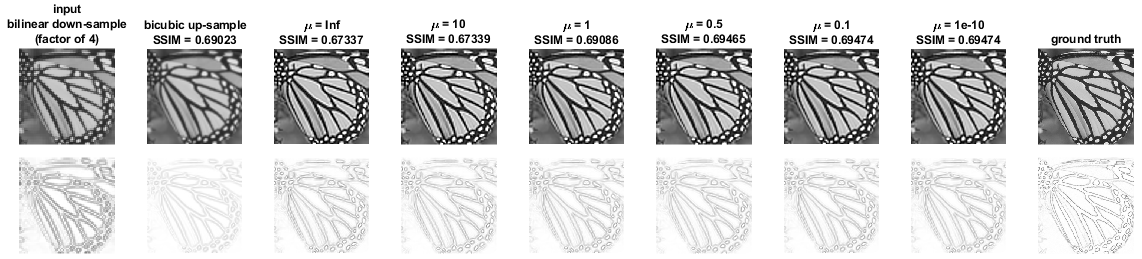
\includegraphics[width=1\textwidth]{mu.png}
	\caption{Image enhancement using the sharpness enhancement function: the reconstructed HR images (top) and inverted gradient magnitude map (bottom). The Structural SIMilarity (SSIM) \cite{ssim04} between the HR image and ground truth increases as $\mu$ gets closer to 0 since the sharpness gets closer to that of the ground truth.}
	\label{fig:mu}
\end{figure}

\subsection{HR Image Reconstruction}

\begin{figure}[H]
	\centering
	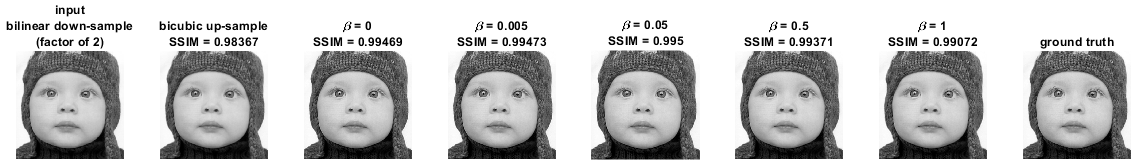
\includegraphics[width=1\textwidth]{beta.png}
	\caption{Effect of changing the value of the parameter $\beta$ towards the SSIM between the reconstructed HR image and the ground truth. We set $\beta = 0.05$, by default, in the implementation. In experiment, the HR images are sharp and clear enough after 25 iterations (default number of iterations in the implementation).}
	\label{fig:beta}
\end{figure}

\begin{figure}[H]
	\centering
	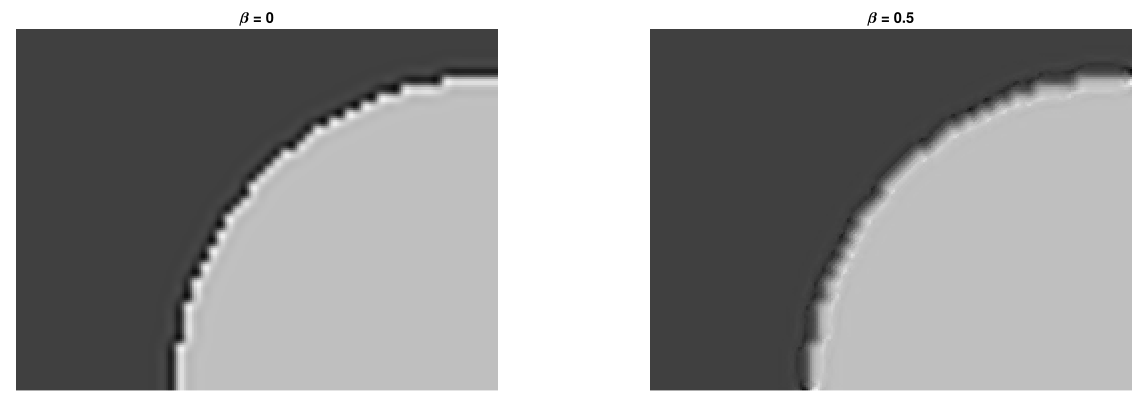
\includegraphics[width=0.7\textwidth]{beta 0 05.png}
	\caption{HR image reconstruction with small and large value of parameter $\beta$. Setting $\beta = 0$ will produce HR image with ringing and jaggy artifacts. On the other hand, the artifacts are less visible when $\beta = 0.5$.}
	\label{fig:beta2}
\end{figure}


\section{Noisy HR Image}

\subsection{Noise Layer}
The SR model using the gradient profile prior is incapable of differing between edge and noise in the image. In other words, the model will treat the noise in the same way as the edge, i.e. enhanced. As an implication, the noise might appear as local maximum in the gradient domain and, in turns, create unexpected gradient profiles. One straightforward solution is to firstly extract the noise layer through a denosing method before applying the HR reconstruction algorithm. This process would remove the unexpected gradient profiles in the image. Secondly, the noise layer is then upsampled and reapplied to the HR image constructed previously. In Figure \ref{fig:sden}, the LR image is denoised with the non-local means algorithm\cite{nlm05} to obtain a more pleasant result to our eye (bottom right) compared to the original result (top right).

\begin{figure}[H]
	\centering
	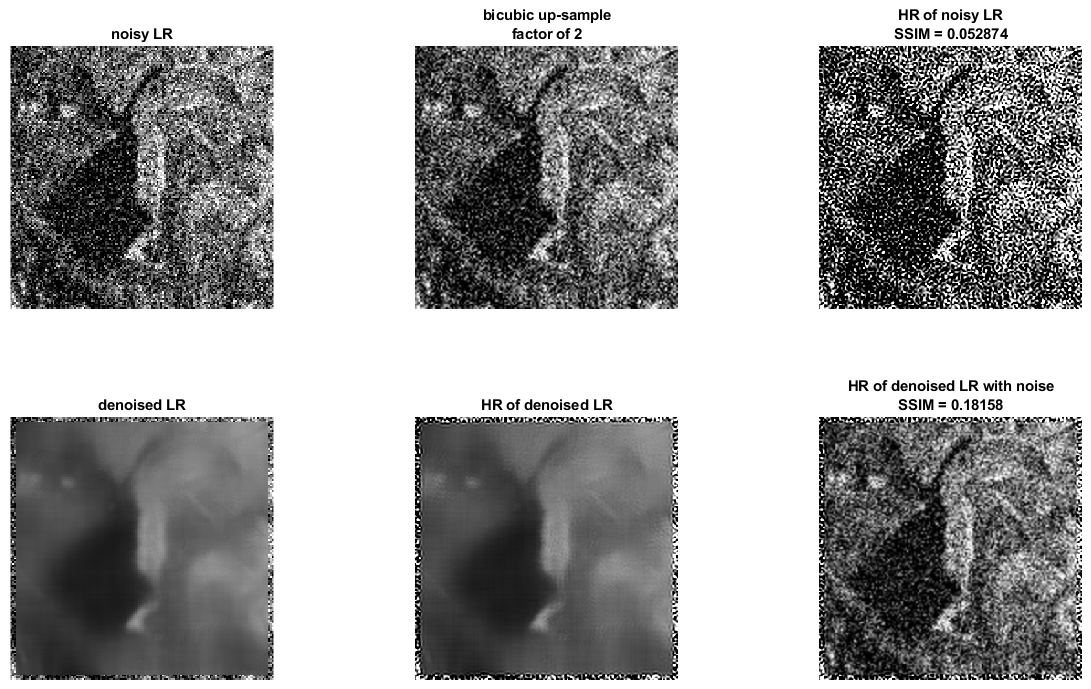
\includegraphics[width=0.8\textwidth]{simple denoise.png}
	\caption{(top) HR image reconstruction from the noisy LR image. (bottom) HR image is reconstructed by adding back the up-sampled noise layer to the HR image generated from the denoised LR image}
	\label{fig:sden}
\end{figure}

\subsection{Convex Combination}


\section{Conclusions}


\begin{thebibliography}{10}

\bibitem{in16} {\sc Yue, Linwei \& Shen, Huanfeng \& Li, Jie \& Yuan, Qiangqiang \& Zhang, Hongyan \& Zhang, Liangpei.} (2016). {\em Image super-resolution: The techniques, applications, and future.} Signal Processing. 128. 10.1016/j.sigpro.2016.05.002. 

\bibitem{sr11} {\sc J. Sun, J. Sun, Z. Xu, \& H. Shum}, {\em Gradient Profile Prior and Its Applications in Image Super-Resolution and Enhancement}, in IEEE Transactions on Image Processing, vol. 20, no. 6, pp. 1529-1542, June 2011.

\bibitem{ssim04} {\sc Zhou Wang, A. C. Bovik, H. R. Sheikh, \& E. P. Simoncelli}, {\em Image quality assessment: from error visibility to structural similarity}, in IEEE Transactions on Image Processing, vol. 13, no. 4, pp. 600-612, April 2004.

\bibitem{nlm05} {\sc A. Buades, B. Coll, \& J. -. Morel}, {\em A non-local algorithm for image denoising}, 2005 IEEE Computer Society Conference on Computer Vision and Pattern Recognition (CVPR'05), San Diego, CA, USA, 2005, pp. 60-65 vol. 2.

\bibitem{noise14} {\sc A. Singh, F. Porikli, \& N. Ahuja}, {\em Super-resolving Noisy Images}, 2014 IEEE Conference on Computer Vision and Pattern Recognition, Columbus, OH, USA, 2014, pp. 2846-2853.

\end{thebibliography}

\end{document}
